\chapter{Основы математической статистики}\label{chap:statistics}\markright{Глава 38}

\section{Выборка и описание данных}
\begin{definition}\term{Генеральная совокупность} (\emph{population}) — изучаемая совокупность объектов или вероятностная модель наблюдений. \par\term{Случайная выборка} (\emph{random sample}) объёма \(n\) — независимые одинаково распределённые величины \(X_1,\ldots,X_n\). После наблюдения получаем числовые данные \(x_1,\ldots,x_n\).\end{definition}
\begin{definition}\term{Статистика} (\emph{statistic}) — измеримая функция выборки, не зависящая от неизвестных параметров. \par\term{Выборочное среднее} (\emph{sample mean}) \(\overline x=\frac1n\sum_{j=1}^n x_j\). \par\term{Эмпирическая функция распределения} (\emph{empirical CDF}) \(F_n(t)=\frac1n\sum_{j=1}^n1_{\{x_j\le t\}}\).\end{definition}
\begin{definition}\term{Медиана выборки} (\emph{sample median}) — среднее по положению значение в упорядоченном ряду; при чётном \(n\) берём полусумму двух центральных. \par\term{Мода} (\emph{mode}) — наиболее часто встречающееся значение; мод может быть несколько. \par\term{Выборочный квантиль} (\emph{sample quantile}) порядка \(0<p<1\) здесь определяется как \(\inf\{t:F_n(t)\ge p\}\). В программах встречаются и другие соглашения с интерполяцией.\end{definition}
\begin{definition}\term{Эмпирическая дисперсия} (\emph{empirical variance}) \(v_n=\frac1n\sum(x_j-\overline x)^2\). \par\term{Исправленная выборочная дисперсия} (\emph{unbiased sample variance}) при \(n\ge2\) есть \(s^2=\frac1{n-1}\sum(x_j-\overline x)^2\).\end{definition}
\par\addvspace{5pt}\begin{lrbox}{\CatFlowBox}\begin{minipage}[t]{\linewidth}
\setlength{\parskip}{5pt}\setlength{\columnsep}{4.5mm}\setlength{\intextsep}{0pt}
\begin{wrapfigure}[13]{r}{54mm}

\includegraphics[width=54mm,height=58mm,keepaspectratio]{images/unique/art-178.png}
\end{wrapfigure}
Одни и те же данные можно описать разными способами. Среднее чувствительно к очень большим значениям, медиана устойчивее к единичным выбросам. Гистограмма показывает частоты по интервалам; при разных ширинах столбцов для сравнения плотностей нужны частоты, делённые на ширину. Описание наблюдённых чисел ещё не доказывает, что выборка представляет интересующую совокупность: способ отбора и зависимость наблюдений влияют на выводы.
\par\WFclear\end{minipage}\end{lrbox}%
\ifdim\dimexpr\ht\CatFlowBox+\dp\CatFlowBox\relax<64mm\dp\CatFlowBox=\dimexpr64mm-\ht\CatFlowBox\relax\fi%
\noindent\usebox{\CatFlowBox}\par\addvspace{5pt}
\section{Оценивание параметров}
\begin{definition}\term{Оценка параметра} (\emph{estimator}) \(T_n\) — статистика, используемая для приближения неизвестного \(\theta\). \par\term{Несмещённость} (\emph{unbiasedness}) означает \(\mathbb E_\theta T_n=\theta\) при каждом допустимом \(\theta\). \par\term{Состоятельность} (\emph{consistency}) означает \(\mathbb P_\theta(|T_n-\theta|>\varepsilon)\to0\) для каждого \(\varepsilon>0\).\end{definition}
\begin{theorem}[Оценки среднего и дисперсии]
Для случайной выборки с конечными средним \(\mu\) и дисперсией \(\sigma^2\): \(\mathbb E\overline X_n=\mu\), \(\operatorname{Var}\overline X_n=\sigma^2/n\); среднее состоятельно. При \(n\ge2\) исправленная дисперсия \(S^2\) несмещённо оценивает \(\sigma^2\), а \(\mathbb EV_n=\frac{n-1}{n}\sigma^2\).
\end{theorem}
\begin{proof}Первые утверждения следуют из линейности, независимости и слабого закона больших чисел. Для дисперсии используем тождество
\[
\sum_{j=1}^n(X_j-\overline X_n)^2=\sum_{j=1}^n(X_j-\mu)^2-n(\overline X_n-\mu)^2.
\]
Ожидание правой части равно \(n\sigma^2-n\cdot\sigma^2/n=(n-1)\sigma^2\). Делим на \(n-1\) или \(n\).\end{proof}
\begin{definition}\term{Функция правдоподобия} (\emph{likelihood}) \(L(\theta)\) — вероятность наблюдённых дискретных данных или значение их совместной плотности как функция параметра \(\theta\). \par\term{Оценка максимального правдоподобия} (\emph{maximum likelihood estimator, MLE}) максимизирует \(L\) по допустимым параметрам.\end{definition}
\begin{theorem}[Максимальное правдоподобие для Бернулли]
Если в \(n\ge1\) независимых испытаниях наблюдалось \(k\) успехов, то оценка \(p\in[0,1]\) максимального правдоподобия равна \(\widehat p=k/n\).
\end{theorem}
\begin{proof}При \(0<k<n\) логарифм правдоподобия равен \(k\ln p+(n-k)\ln(1-p)\). Его производная \(k/p-(n-k)/(1-p)\) обращается в нуль при \(p=k/n\); вторая производная отрицательна. На границах правдоподобие равно нулю. При \(k=0\) функция \((1-p)^n\) максимальна в \(0\), при \(k=n\) функция \(p^n\) максимальна в \(1\).\end{proof}
\section{Доверительные интервалы}
\begin{definition}\term{Доверительный интервал} (\emph{confidence interval}) уровня \(1-\alpha\), \(0<\alpha<1\), — случайный интервал \([L(X),U(X)]\), удовлетворяющий \(\mathbb P_\theta(L\le\theta\le U)\ge1-\alpha\) для всех параметров модели. Уровень относится к процедуре при повторении выборки. После наблюдения параметр фиксирован, а границы стали числами.\end{definition}
\par\addvspace{5pt}\begin{lrbox}{\CatFlowBox}\begin{minipage}[t]{\linewidth}
\setlength{\parskip}{5pt}\setlength{\columnsep}{4.5mm}\setlength{\intextsep}{0pt}
\begin{wrapfigure}[9]{l}{54mm}
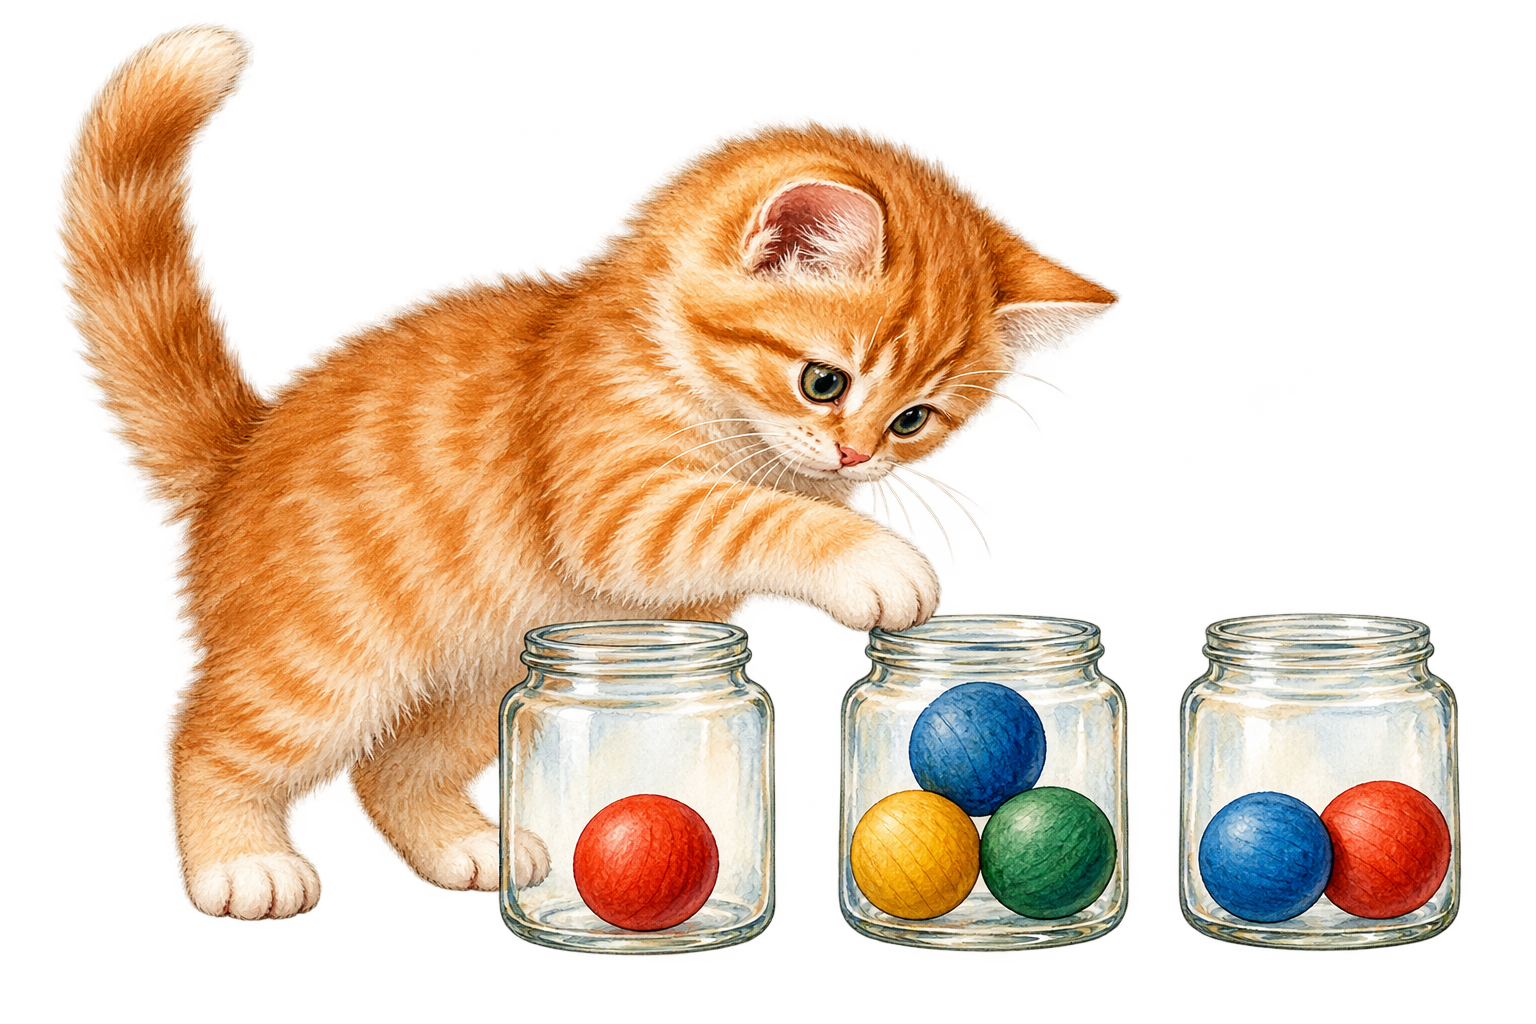
\includegraphics[width=54mm,height=58mm,keepaspectratio]{images/unique/art-179.png}
\end{wrapfigure}
Доверительный уровень описывает покрытие в повторных опытах при выполнении предположений модели. Узкий интервал, полученный по смещённой выборке, не исправляет способ отбора данных. Для малых выборок важен точный закон статистики; замена его нормальным распределением требует отдельного обоснования. Увеличение числа наблюдений уменьшает случайную погрешность среднего, если наблюдения действительно независимы.
\par\WFclear\end{minipage}\end{lrbox}%
\ifdim\dimexpr\ht\CatFlowBox+\dp\CatFlowBox\relax<64mm\dp\CatFlowBox=\dimexpr64mm-\ht\CatFlowBox\relax\fi%
\noindent\usebox{\CatFlowBox}\par\addvspace{5pt}
\begin{theorem}[Точный интервал для нормального среднего при известной дисперсии]
Для независимых \(X_j\sim\operatorname N(\mu,\sigma^2)\), где \(\sigma>0\) известно, и \(z=\Phi^{-1}(1-\alpha/2)\) интервал
\[
\left[\overline X_n-z\frac\sigma{\sqrt n},\ \overline X_n+z\frac\sigma{\sqrt n}\right]
\]
имеет покрытие ровно \(1-\alpha\). Для \(\alpha=0{,}05\) приближённо \(z=1{,}96\).
\end{theorem}
\begin{proof}Сумма независимых нормальных величин нормальна, поэтому \(Z=\sqrt n(\overline X_n-\mu)/\sigma\sim\operatorname N(0,1)\). Это свойство сумм получается свёрткой нормальных плотностей: в показателе произведения выделяется полный квадрат, а интеграл оставшегося гауссова множителя даёт нормировочную константу. Симметрия стандартной нормали даёт \(\mathbb P(-z\le Z\le z)=1-\alpha\). Преобразуем двойное неравенство к границам для \(\mu\).\end{proof}
\begin{theorem}[Центральная предельная теорема; central limit theorem]
Если \(X_j\) независимы, одинаково распределены и имеют конечные среднее \(\mu\), дисперсию \(0<\sigma^2<\infty\), то для каждого \(t\in\mathbb R\)
\[
\mathbb P\!\left(\frac{\sqrt n(\overline X_n-\mu)}\sigma\le t\right)\longrightarrow\Phi(t).
\]
\end{theorem}
Общее доказательство центральной предельной теоремы выходит за рамки этого введения. Она обосновывает нормальное приближение при больших \(n\), но не даёт универсального конечного порога «достаточно большой выборки» без дополнительных условий. Используем без доказательства два дополнительных результата: при конечном втором моменте \(S^2\) состоятельно оценивает \(\sigma^2\); теорема Слуцкого разрешает соответствующую замену нормировки. При неизвестной \(\sigma\) замена на \(S\) поэтому даёт асимптотический интервал при указанных предположениях; его покрытие приближённое. Для нормальной выборки точный интервал с неизвестной дисперсией использует распределение Стьюдента и требует отдельного изучения.
\begin{theorem}[Гарантированный интервал для доли успехов]
Для \(n\) независимых испытаний Бернулли и \(\widehat p=k/n\) положим \(d=1/(2\sqrt{n\alpha})\). Интервал \([\widehat p-d,\widehat p+d]\cap[0,1]\) покрывает \(p\) с вероятностью не меньше \(1-\alpha\).
\end{theorem}
\par\addvspace{5pt}\begin{lrbox}{\CatFlowBox}\begin{minipage}[t]{\linewidth}
\setlength{\parskip}{5pt}\setlength{\columnsep}{4.5mm}\setlength{\intextsep}{0pt}
\begin{wrapfigure}[11]{l}{54mm}

\includegraphics[width=54mm,height=58mm,keepaspectratio]{images/unique/art-181.png}
\end{wrapfigure}
\textit{Доказательство.} Поскольку \(\operatorname{Var}\widehat p=p(1-p)/n\le1/(4n)\), неравенство Чебышёва даёт \(\mathbb P(|\widehat p-p|\ge d)\le\alpha\). Значит, интервал покрывает \(p\) хотя бы с нужной вероятностью. Пересечение с \([0,1]\) не теряет допустимых значений параметра.\hfill\(\blacksquare\)
\par\WFclear\end{minipage}\end{lrbox}%
\ifdim\dimexpr\ht\CatFlowBox+\dp\CatFlowBox\relax<64mm\dp\CatFlowBox=\dimexpr64mm-\ht\CatFlowBox\relax\fi%
\noindent\usebox{\CatFlowBox}\par\addvspace{5pt}

\section{Гипотезы и p-значение}
\begin{definition}\term{Нулевая гипотеза} (\emph{null hypothesis}) \(H_0\) задаёт проверяемую модель. \par\term{Альтернативная гипотеза} (\emph{alternative hypothesis}) \(H_1\) описывает отклонение от неё. \par\term{Ошибка первого рода} (\emph{type I error}) — отклонение верной \(H_0\). \par\term{Уровень значимости} (\emph{significance level}) \(\alpha\) ограничивает вероятность такой ошибки при \(H_0\).\end{definition}
\begin{definition}\term{p-значение} (\emph{p-value}) для заданной статистики и направления отклонения — вероятность при \(H_0\) получить столь же или более экстремальное значение статистики. Для составной \(H_0\) нужна процедура, корректная для всех её допустимых параметров. При \(p\text{-value}\le\alpha\) заранее выбранный критерий отклоняет \(H_0\).\end{definition}
При проверке честной монеты против альтернативы «успех чаще половины» девять успехов из десяти дают \(\mathbb P_{1/2}(K\ge9)=11/1024\). Это вероятность такого или более крайнего результата при честной монете. Она не равна вероятности честности монеты после наблюдения. Неотклонение гипотезы тоже не доказывает её: данных может быть мало, а критерий может плохо различать близкие альтернативы.

\section{Корреляция и линейная регрессия}
\begin{definition}Для пар данных \((x_j,y_j)\) положим \(S_{xx}=\sum(x_j-\overline x)^2\), \(S_{yy}=\sum(y_j-\overline y)^2\), \(S_{xy}=\sum(x_j-\overline x)(y_j-\overline y)\). \term{Выборочная корреляция Пирсона} (\emph{Pearson sample correlation}) \(r=S_{xy}/\sqrt{S_{xx}S_{yy}}\) определена при \(S_{xx}S_{yy}>0\).\end{definition}
\begin{definition}\term{Метод наименьших квадратов} (\emph{ordinary least squares, OLS}) выбирает прямую \(y=a+bx\), минимизирующую \(\sum(y_j-a-bx_j)^2\).\end{definition}
\begin{theorem}[Формулы корреляции и регрессии]
Корреляция удовлетворяет \(|r|\le1\). Если \(S_{xx}>0\), единственная прямая наименьших квадратов имеет
\[
b=\frac{S_{xy}}{S_{xx}},\qquad a=\overline y-b\overline x.
\]
\end{theorem}
\begin{proof}Граница для \(r\) есть неравенство Коши—Буняковского для векторов центрированных наблюдений. Сумма квадратов раскладывается как
\[
 n(a+b\overline x-\overline y)^2+S_{yy}-2bS_{xy}+b^2S_{xx}.
\]
Первый квадрат минимален при \(a=\overline y-b\overline x\); выделение квадрата по \(b\) даёт единственный минимум при \(S_{xx}>0\).\end{proof}
\par\addvspace{5pt}\begin{lrbox}{\CatFlowBox}\begin{minipage}[t]{\linewidth}
\setlength{\parskip}{5pt}\setlength{\columnsep}{4.5mm}\setlength{\intextsep}{0pt}
\begin{wrapfigure}[11]{r}{54mm}

\includegraphics[width=54mm,height=58mm,keepaspectratio]{images/unique/art-180.png}
\end{wrapfigure}
Корреляция измеряет линейную связь. Нулевая корреляция не исключает нелинейную зависимость, а высокая корреляция не устанавливает причину. Прямая регрессии описывает выбранные данные; прогноз за пределами наблюдённого диапазона требует отдельной модели. Сначала полезно нарисовать точки, заметить выбросы и форму зависимости, затем вычислять коэффициенты.
\par\WFclear\end{minipage}\end{lrbox}%
\ifdim\dimexpr\ht\CatFlowBox+\dp\CatFlowBox\relax<64mm\dp\CatFlowBox=\dimexpr64mm-\ht\CatFlowBox\relax\fi%
\noindent\usebox{\CatFlowBox}\par\addvspace{5pt}
% END-STATISTICS-THEORY

\par\noindent\begin{minipage}{\linewidth}\section*{Графики}
\begin{center}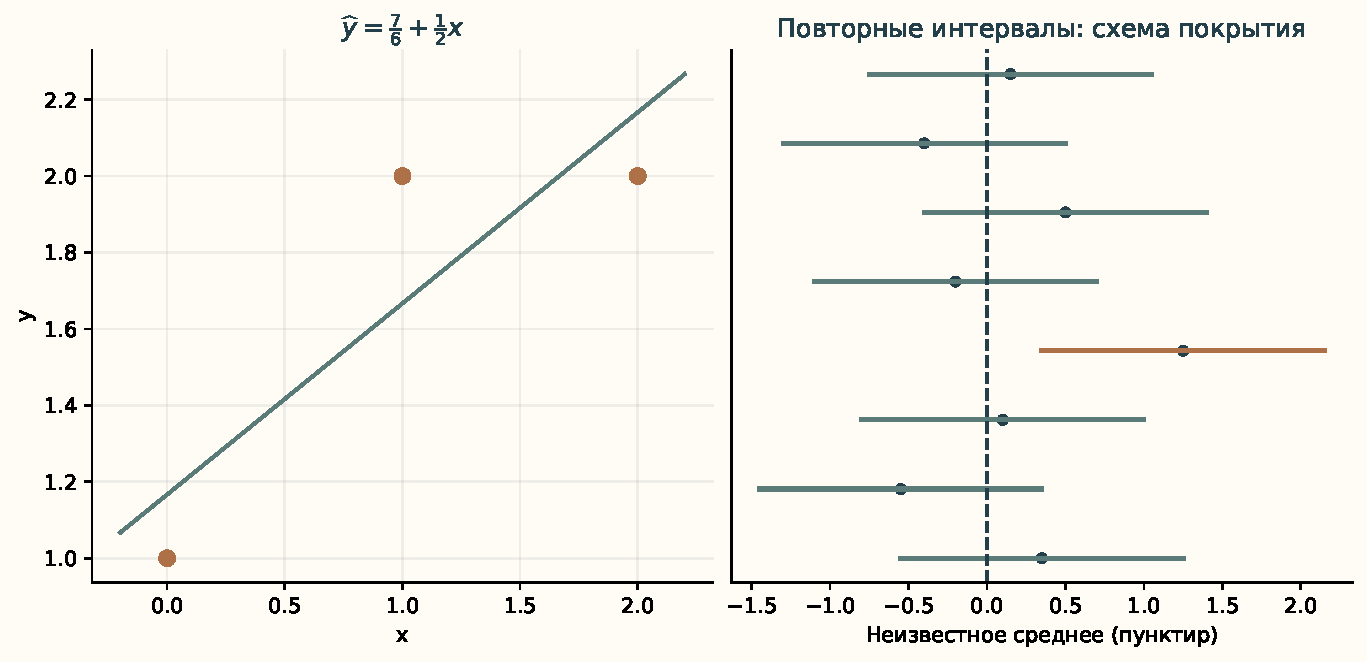
\includegraphics[width=\textwidth,height=.79\textheight,keepaspectratio]{images/atlas-statistics.pdf}\par\small Данные, регрессия и доверительные интервалы\end{center}\end{minipage}\par
\Needspace{7\baselineskip}\section*{Задачи}
\begingroup\setlength{\parskip}{1pt}
\noindent\begin{minipage}[t]{\linewidth}\textbf{38.1.} Для данных \(1,2,3,4\) найди среднее, медиану, \(v_n\) и \(s^2\).\par\end{minipage}\par
\noindent\begin{minipage}[t]{\linewidth}\textbf{38.2.} Для данных \(1,1,2,4,7\) найди моду, медиану, среднее и квантиль порядка \(\dfrac34\) по определению этой главы.\par\end{minipage}\par
\noindent\begin{minipage}[t]{\linewidth}\textbf{38.3.} Для данных \(1,2,3,4\) найди \(F_n(0),F_n(2),F_n(2{,}5),F_n(4)\).\par\end{minipage}\par
\noindent\begin{minipage}[t]{\linewidth}\textbf{38.4.} В выборке \(1,2,3,4,5\) заменили \(5\) на \(105\). Как изменились среднее и медиана?\par\end{minipage}\par
\noindent\begin{minipage}[t]{\linewidth}\textbf{38.5.} Почему для исправленной дисперсии требуется \(n\ge2\)?\par\end{minipage}\par
\par\addvspace{5pt}\begin{lrbox}{\CatFlowBox}\begin{minipage}[t]{\linewidth}
\setlength{\parskip}{5pt}\setlength{\columnsep}{4.5mm}\setlength{\intextsep}{0pt}
\begin{wrapfigure}[9]{r}{54mm}

\includegraphics[width=54mm,height=58mm,keepaspectratio]{images/unique/art-182.png}
\end{wrapfigure}
\textbf{38.6.} Наблюдения независимы и имеют дисперсию \(16\). Найди дисперсию среднего при \(n=25\) и его стандартное отклонение.\par

\textbf{38.7.} В \(20\) независимых испытаниях было \(7\) успехов. Найди оценку максимального правдоподобия вероятности успеха.\par

\textbf{38.8.} В \(8\) испытаниях успехов нет. Чему равна MLE? Следует ли из этого, что истинное \(p=0\)?\par

\textbf{38.9.} Нормальная выборка имеет \(n=100\), \(\overline x=10\); известно \(\sigma=2\). Построй приближённые числовые границы точного 95\%-го доверительного интервала, используя \(z\approx1{,}96\).\par
\par\WFclear\end{minipage}\end{lrbox}%
\ifdim\dimexpr\ht\CatFlowBox+\dp\CatFlowBox\relax<64mm\dp\CatFlowBox=\dimexpr64mm-\ht\CatFlowBox\relax\fi%
\noindent\usebox{\CatFlowBox}\par\addvspace{5pt}

\noindent\begin{minipage}[t]{\linewidth}\textbf{38.10.} Во сколько раз изменится полуширина интервала для среднего при увеличении объёма независимой выборки в \(4\) раза и той же известной дисперсии?\par\end{minipage}\par
\noindent\begin{minipage}[t]{\linewidth}\textbf{38.11.} Какого числа испытаний достаточно по оценке Чебышёва, чтобы ошибка доли успехов была меньше \(0{,}1\) с вероятностью не меньше \(0{,}95\), независимо от \(p\)?\par\end{minipage}\par
\noindent\begin{minipage}[t]{\linewidth}\textbf{38.12.} Наблюдалось \(60\) успехов из \(100\). Найди гарантированный интервал из теоремы при \(\alpha=0{,}05\).\par\end{minipage}\par
\noindent\begin{minipage}[t]{\linewidth}\textbf{38.13.} Монету проверяют против альтернативы \(p>\dfrac12\). При \(9\) успехах из \(10\) найди одностороннее p-значение. Отклоняется ли \(H_0:p=\dfrac12\) при \(\alpha=0{,}05\)?\par\end{minipage}\par
\noindent\begin{minipage}[t]{\linewidth}\textbf{38.14.} В той же проверке получено \(8\) успехов из \(10\). Найди p-значение и решение при \(\alpha=0{,}05\).\par\end{minipage}\par
\noindent\begin{minipage}[t]{\linewidth}\textbf{38.15.} Что является ошибкой первого рода в проверке честности монеты?\par\end{minipage}\par
\noindent\begin{minipage}[t]{\linewidth}\textbf{38.16.} Можно ли p-значение \(0{,}03\) назвать вероятностью истинности нулевой гипотезы?\par\end{minipage}\par
\noindent\begin{minipage}[t]{\linewidth}\textbf{38.17.} Для точек \((0,1),(1,2),(2,2)\) найди прямую наименьших квадратов.\par\end{minipage}\par
\noindent\begin{minipage}[t]{\linewidth}\textbf{38.18.} Для тех же трёх точек найди корреляцию.\par\end{minipage}\par
\noindent\begin{minipage}[t]{\linewidth}\textbf{38.19.} Для точек \((-1,1),(0,0),(1,1)\) найди корреляцию. Есть ли зависимость между координатами?\par\end{minipage}\par
\noindent\begin{minipage}[t]{\linewidth}\textbf{38.20.} В данных все \(x_j\) одинаковы. Определены ли корреляция и единственный наклон регрессии?\par\end{minipage}\par
\noindent\begin{minipage}[t]{\linewidth}\textbf{38.21.} Докажи тождество \(\sum(x_j-\overline x)^2=\sum x_j^2-n\overline x^2\).\par\end{minipage}\par
\noindent\begin{minipage}[t]{\linewidth}\textbf{38.22.}\starmark{} Выведи \(\mathbb EV_n=\dfrac{n-1}{n}\sigma^2\) и объясни поправку \(n-1\).\par\end{minipage}\par
\noindent\begin{minipage}[t]{\linewidth}\textbf{38.23.} Докажи, что прямая наименьших квадратов с \(S_{xx}>0\) проходит через \((\overline x,\overline y)\).\par\end{minipage}\par
\noindent\begin{minipage}[t]{\linewidth}\textbf{38.24.}\starmark{} Для фиксированного \(t\) докажи несмещённость \(F_n(t)\) как оценки \(F(t)\) и найди её дисперсию при независимой выборке.\par\end{minipage}\par
\endgroup
